\chapter[Introduction]{Introduction} \label{ch:1_intro}

We elaborate on both field-theoretic and quantum mechanical descriptions of (non-)Abelian anyons, emphasizing the role of contact interaction terms. Field theoretic contact terms, required for the sake of renormalizability in general, implement the self-adjoint extension of the quantum mechanical Hamiltonian~\cite{Lee1997}.



\begin{figure}[tb]
\centering
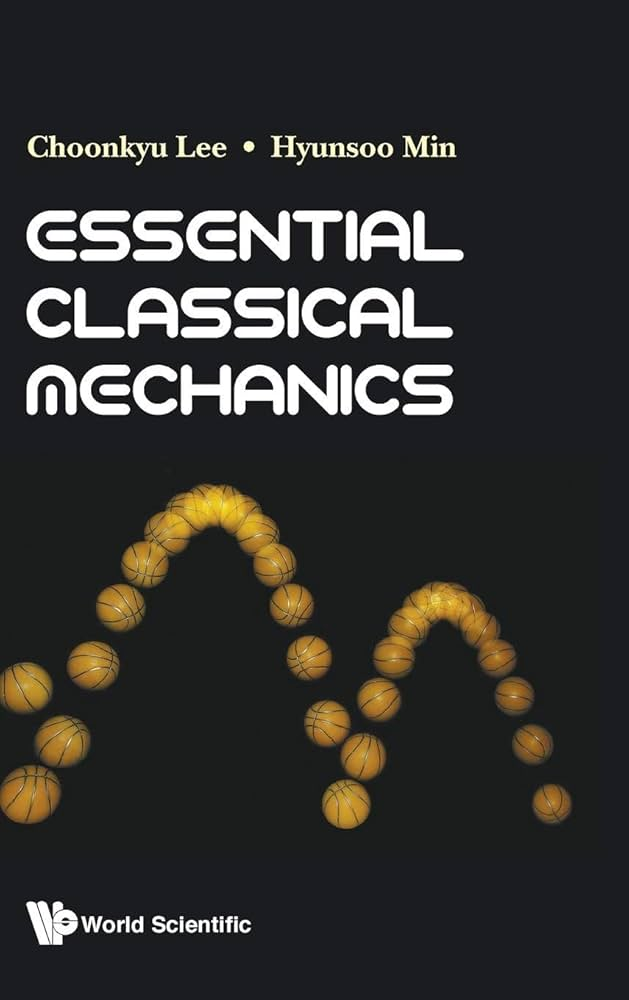
\includegraphics[width=0.6\linewidth]{figures/mechanics.jpg}
\caption[Essential Classical Mechanics]{
	This is a book on intermediate classical mechanics.
	In this book, classical mechanics is presented as a useful tool to analyze the physical universe and also as the base on which the whole pyramid of modern physics has been erected. 
	Various mechanical concepts are developed in a highly logical manner, with relatively thorough treatments on mathematical procedures and many physically interesting applications. 
	Connections to more modern theoretical developments (including statistical physics, relativity, and quantum mechanics) are emphasized~\cite{Lee2018Book}.
}
\label{fig:plph_GaAs}
\end{figure}